
This section will first introduce the company Visual Solutions\footnote{http://www.bbvisuals.com/} who provided the practical problem. Secondly I will give a quick overview of how the application Virtual Arena works by describing its underlying architecture, then I will look at how the enterprise firewall works, and lastly look some of the security concerns that occur when a enterprise collaboration system has to access the public internet.

\section{Visual Solutions}
Visual Solutions is a Norwegian company in the BB Visual Group\footnote{http://www.bbvisualgroup.com/}. Their primary business is within the integration of operations for the oil and gas industry. They create solutions enabling collaboration across organisation units and geographic locations. One of their applications Virtual Arena\cite{solutions_b2_virtual_2014}, which from now on will be referred to as VA, is a powerful and interactive tool that allows for high-performance application sharing, with audio and video communication from a 3D shared scene\ref{fig:?}. VA supports many-to-many collaborative scenarios by utilizing a media server which will be described in the next section. 

\section{Virtual Arena}
VA is the application that Visual Solutions has created for doing visual collaboration\cite{VirtualArena} over IP. The architecture of VA is visualized in Figure\ref{?}. The application uses a media server that serves multiple purposes. It acts as a \gls{mcu}, applies mitigation strategies for scenarios with limited bandwidth, and also sharing of applicaton data. Mitigation strategies can f.ex be reducing the video bitrate to adjust adapt for a poor connection. The media server works together with a router for distributing the streams. By utilizing a media server VA can support a lot incoming and outgoing streams. A client can subscribe to multiple streams of audio/video and applications. It manages these connections using a tree structure, but this is an advanced topic that I won't go into detail about. In the next subsections the different parts of the architecture\ref{?} will be described with the necessary information required to understand the practical problem this thesis will try to solve. 
\\
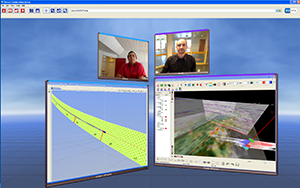
\includegraphics[scale=0.6]{virtualarena.png}
\\
\\

\subsection{Signaling}
VA has a proprietary way of doing signaling over RTCP. RTCP is control protocol for RTC. This is where the clients send messages to the media server describing which streams they want to subscribe to. Communication between peers and the media server is done by opening up ports in the firewall to listen for incoming TCP and UDP connections. These ports are preconfigured for the application. The media server can receive incoming streams and route it to all peers connected. The streams are identified using a SSRC, which is defined in the header packets of the RTP streams.

\subsection{Transport layer}
VA uses raw RTP stream over UDP. This is basically the most standard protocol used for transmitting real-time data in enterprise communication systems\cite{}.

\subsection{Media}
VA uses free and open source codecs for audio and video. It uses Speex for audio, and Theora for video. These are not the most commonly used codec, as the g.711 for audio and H.264 for video are the most common ones. Even though H.264 is licensed by Ericsson, it offers the added benefits of hardware acceleration in a lot of graphic cards, and is also one of the best codecs for real-time streaming as of now\cite{source}.

%%are common in, but h.264 g.711 standard in ims systems%%

\subsection{Security}
VA only uses raw UDP streams because nothing more is needed. It operates in a closed business environement, so transport level encryption is not needed, because unidentified peers are not allowed inside the network anyways. The enterprise firewall has very strict policys, only allowing certain kinds of traffic.?????

\subsection*{Summary}
VA operates like a typical enterprise comunication system. CODEC?? 